% !TeX encoding = UTF-8
% !TeX root = V6_SAXS.tex
% !TeX spellcheck = en_US

\section{Theory}

\subsection{Introduction}
The aim of this experiment is to determine internal structures of solids with help of X-Ray scattering. In the experiment, we use several techniques to achieve this goal: Frontscattering, backscattering, and the Guinier setup. The analysed solids include mono-crystalline (e.g. a silicon wafer), poly-crystalline (e.g. silicon powder), semi-crystalline (polymer) and amorphous samples.

\subsection{X-Rays}
	X-Rays are electromagnetic waves in an interval of high energies and thus wavelengths in the range of $\SI{0.1}{\nano\metre}-\SI{10}{\nano\metre}$. To use such waves for determining structures of crystallized solids with long range order one has to choose his wavelength in range of sample lattice values.\\
	X-Rays can be generated with thermal activated electrons which radiate high energetic photons after interaction with matter. This principle of negative acceleration is called Bremsstrahlung. For this purpose generated and usually accelerated electrons are forced to hit a target like aluminium or copper. Immediately after hitting the target the electrons emit a high energetic photon to fulfill the principles of momentum and energy conservation. The wavelength of Bremsstrahlung is given by
	\begin{equation}
		\lambda_\text{min}=\frac{hc}{eU}~\mathrm{,}
	\end{equation}
	where $h$ is the Planck constant, $c$ the velocity of light\footnote{If not in vacuum, the velocity is corrected by the formula  $c=\frac{c_0}{n}$, where $n$ is the refraction index.}, $e$ the elementary charge and $U$ the acceleration voltage. 
	The spectra of X-Rays are continuous. Further there exist sharp discrete emission lines. A example spectrum is given in figure \ref{Bremsspektrum}
	\begin{figure}[h]
		\centering
		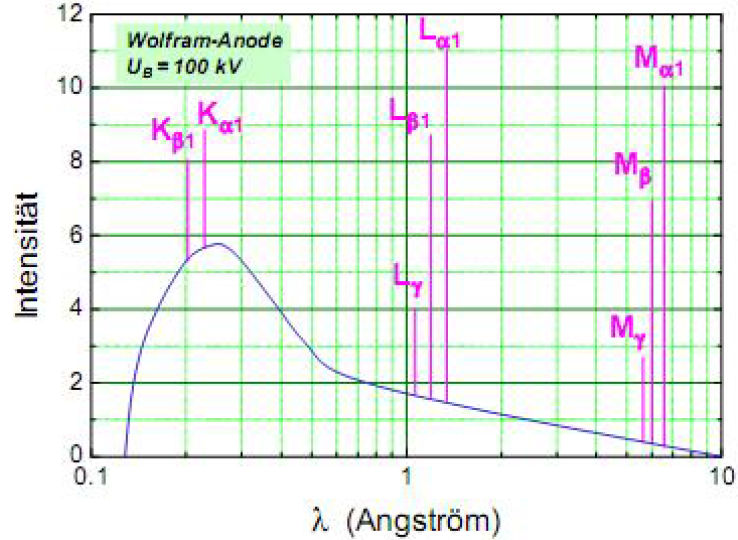
\includegraphics[width=0.8\textwidth]{Bemsstrahlung.png}
		\caption[Example of an X-Ray spectrum]{Example of an X-Ray spectrum. The wavelength axis is given in logarithmic scale. The spectrum is from an X-Ray tube with wolfram anode. The variables $K,L,M$ represent the starting orbit. The first index gives the transition between the orbits, in which e.g. $\alpha$ is a quantum number change from $n=1\to m=2$. The last index gives the ending level of the fine structure. \cite{lit:GroMa14}}
		\label{Bremsspektrum}
	\end{figure}
	The discrete lines are created through interactions with the accelerated electron and the orbit electrons of the latter. The process is an impact of the accelerated electrons to low orbit electrons. Usually one hits out the s or p Orbital electron out. Immediately after the striking out the bound electron another electron from a higher orbit relaxes down to the empty orbit. The nomenclature for the first three orbits are $K, L, M$ for the Orbit. The sign $K$ represents the orbit s (quantum number n=1, l=0), $L$ the orbit p (quantum number n=2, l=-1,0,1) and $M$ the orbit d (quantum number n=3, l=-2,-1,0,1,2). The next sign is given in the Index of the starting orbit and represents the transition between start and end orbit. Therefor a change from $K$ to the next higher Orbit $L$ would be signed with a $\alpha$. For higher Orbits jumps one can follow the Greek alphabet. The last index shows the ending level in the fine structure. A quantitative representation of X-Ray is given by Moseleys law:
	\begin{equation}
		\frac{1}{\lambda}=R(Z-K)^2 \left ( \frac{1}{n^2} - \frac{1}{m^2} \right )
	\end{equation}
	in which $\lambda$ is the wavelength, $R$ the Rydberg constant, $Z$ the ordinal number, $K$ a experimentally measured shielding constant, $n$ quantum number of the starting orbit and $m$ the ending orbit.
	
	\subsection{X-Ray scattering}
	Solid samples are build up with crystals. Each crystal is defined with a periodically lattice and his atomic basis. In general their exits 14 different elementary lattices, which are named Bravais Lattices. The Basis is given as a natural number filling up the elementary lattice. Further crystals can posses properties like long range or short range order. Notice that polycrystalline structure is described with a short range order. For example amorphous structure don't underlie a periodically order of crystal lattices.
	
	\subsubsection{Laue-Condition}
	The Laue-Condition is a general expression for constructive interference in scattering problems. With this constraint, only multiple integers of the scattering waves are allowed. If we define the normalized unit vectors $\vec s$ as incident beam, $\vec s_0$ as scattered beam and $\vec {a_1}$ as real lattice vector, one can find the Laue-Condition as following expression:
	\begin{equation}
		\vec{a_1} \cdot (\vec s - \vec{s_0})=m \lambda ~~~~~~~ m\in \mathbb{Z}~\mathrm{.}
	\end{equation}
	With help of two further unit vector equations, the Laue-Condition is generalized to three dimensions. If all three are fulfilled, one gets scattering reflexes. Just by replacing the unit vectors $s~\mathrm{and}~s_0$ with the wave vector $\vec k$ and the property $|\vec k|=\frac{2\pi}{\lambda}$ the three Laue equations gets simplified to one equation in form:
	\begin{equation}
		\vec k - \vec {k_0}=\vec G ~\mathrm{,}
		\label{laue}
	\end{equation}
	whereat $\vec G$ is the reciprocate lattice vector. The equation \ref{laue} can be expressed alternative as Ewald construction. Figure \ref{fig:ewald} shows this construction on a two dimensional rectangular lattice. One can see immediately the equation \eqref{laue} is hold for a sphere. The construction rule is following. One has to start with the incident beam wave vector $\vec k$ and let it end on a lattice point. The next step is to draw a sphere centered on the starting point with radius $\vec{k}$. Now all lattice points which are exactly or almost on the sphere can be observed in the measurement and are the scattered wave vector $\vec {k_0}$. The connection of the ends of incident and scattered beam yields to the reciprocal wave vector $\vec G$. Notice that for X-Rays the Ewald sphere radius is getting much bigger than for visible light.
	\begin{figure}[h]
		\centering
		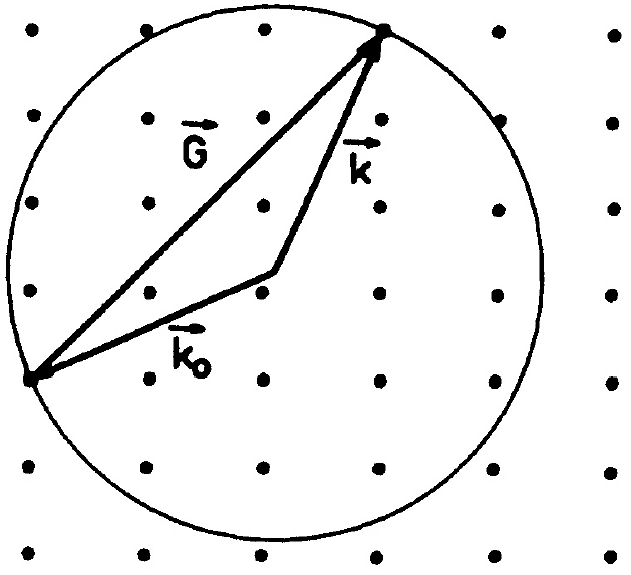
\includegraphics[width=0.8\textwidth]{ewald.png}
		\caption[Ewald sphere for a two dimensional lattice]{Ewald sphere for a two dimensional lattice. \cite{Kop}}
		\label{fig:ewald}
	\end{figure}
	
	\subsubsection{Bragg-Condition}
	
	Braggs formulation of scattering is a alternative but equivalent way to describe scattering reflexes. Thus notice that the reciprocal wave vector $\vec G$ is written in form of:
	\begin{equation}
		\vec G= h\vec{b_1}+k\vec{b_2}+l\vec{b_3}
	\end{equation}
	and is perpendicular to the lattice plane, which is given by the three Miller indices's ($hkl$). The distance between lattices planes are given by:
	\begin{equation}
		d_{hkl}=\frac{2\pi}{|\vec{G}|}.
	\end{equation}
	At the following calculation we define $\vec G$ in form:
	\begin{equation}
		\vec G = n \cdot \vec g = n(h\vec{b_1}+k\vec{b_2}+l\vec{b_3})~\mathrm{.}
	\end{equation}
	The variable $n$ is a positive integer. The Laue equation \ref{laue} changes to the form:
	\begin{equation}
		\vec{s}-\vec{s_0}=n \frac{\lambda}{2 \pi}\vec g
	\end{equation}
	From figure \ref{fig:Bragg} it is obvious that the vectors $\vec s,\vec{s_0}$ and $\vec g$ build up a equal sided triangle. With help of the property that $\vec{G} \perp (hkl)$ follows the left handed side of \ref{laue}
	\begin{equation}
		\mathrm{sin}(\theta)=\frac{1}{2} n \frac{\lambda}{2\pi}|\vec g|~\mathrm{.}
	\end{equation}
	With the identity $|\vec g|= \frac{2\pi}{d_{hkl}}$ follows the Braggs condition:
	\begin{equation}
		2d_{hkl} \mathrm{sin}(\theta)=n \lambda~\mathrm{.}
	\end{equation}
	
	\subsubsection{General scattering theory}
	
	Now we consider a case in which a far away source $Q$ is radiating X-Ray to a sample at position $P$. At $P$ we can estimate planar X-Ray waves. Now the planar wave $\Psi_0$ scatters there. From this scattering point follows a spherical wave which we detect at the observation point $B$. Microscopically we force the electrons of one atoms in point $P$ to an oscillation. Therefore the wave description in $P$ is:
	\begin{equation}
		\Psi_P(\vec r)= \Psi_0 e^{\boldsymbol{i}\vec k (\vec R+\vec r)}~\mathrm{,}
	\end{equation}
	with $\vec R$ is the lattice vector. The detected spherical waves in $B$ are given by
	\begin{equation}
		\Psi_B(\vec r)= \frac{\Psi_P \rho(\vec r)}{|\vec R- \vec r|}e^{\boldsymbol{i}\vec k' (\vec R - \vec r)}~\mathrm{.}
		\label{detek}
	\end{equation}
	The quantity $\rho(\vec r)$ gives the electron density and $k'$ is the scattered wave vector. Now we notice that the distance between sample and detector is much larger as the lattice distance and the scattered wave vector $\vec k'$ is almost parallel to $(\vec R-\vec r)$. Therefor we can approximate equation \ref{detek} to the form:
	\begin{equation}
		\Psi_B(\vec{r})=\Psi_P \rho(\vec r) \frac{e^{\boldsymbol{i}\vec {k'} \cdot (\vec R-\vec r)}}{\vec R}~\mathrm{.}
	\end{equation}
	To get the scattering intensity for the whole crystal, one needs to integrate over the volume, which includes all lattice points. Therefore mathematically the intensity is given by:
	\begin{equation}
		I(\Delta \vec k)\propto |\Psi_B|^2\propto \left| \int \rho(\vec r) e^{-\boldsymbol{i}\Delta \vec k \cdot \vec r}d^3r \right|
	\end{equation}
	Usually lattice of a solid can be describes over a sum of Delta Distributions, alternatively named as Delta comb. This sum is in the from:
	\begin{equation}
		g(\vec r)=\sum_{\vec R}=\delta(\vec r -\vec R)~\mathrm{,}
		\label{deltakamm}
	\end{equation}
	in which $\vec R$ is the lattice point position. The diffraction can be computed by a convolution of lattice function \ref{deltakamm} and a diffraction function, which we call here $\rho_B$. In respect to the convolution theorem we can express the diffraction pattern with:
	\begin{equation}
		\Psi_B \propto \mathrm{FT}(g \times \rho_B)=\mathrm{FT}(g) \cdot \mathrm{FT}(\rho_B)~\mathrm{.}
	\end{equation}
	Further we can express equation \ref{deltakamm} with his Fourier transformed as 
	\begin{equation}
			\mathrm{FT}(\rho_B (\vec r))=\sum_{\vec R} e^{-\boldsymbol{i} \Delta \vec k \vec R}=	
			\begin{cases}
			
			N	& \text{for } \Delta \vec k = \vec G \\
			0	& \text{for } \Delta \vec k \neq \vec G
			
			\end{cases}
	\end{equation}
	To handle the full diffraction pattern, one needs to introduce Structure factors. The Structure factor gives the condition of constructive interference relying on e.g. atomic position and shape constrains. The factor can be expressed in his Fourier transformed expression and is in the form:
	\begin{equation}
			S_G = \mathrm{FT}(\rho_B(\vec r))= \int_{Cell} \rho_B(\vec r) e^{-\boldsymbol{i} \vec G \vec r}d^3 r~\mathrm{.}
	\end{equation}
	Further the atomic form factors can be expressed analogously. Therefor the scattering function is convoluted with the atomic function $\rho_a^j$. The index $j$ represents the j-th atom. The structure factor can be redefined as
	\begin{equation}
		S_G= \sum_j \mathit{f}_j e^{-\boldsymbol{i} \vec G \cdot \vec {r}_j}
	\end{equation}
	and with the atomic form factor
	\begin{equation}
		\mathit{j}_j=\mathrm{FT}(\rho^j_A)=\int_{Atom}=\rho^j_A e^{-\boldsymbol{i}\vec G \cdot \vec{r'}}d^3r'~\mathrm{.}
	\end{equation}
	The variable $\vec{r}'$ represents the position inside of the j-th atom. The structure factor influence diffraction reflexes sufficiently.

	\section{Experimental Setup}
	\subsection{Laue method}
	
	\begin{figure}[h]
		\centering
		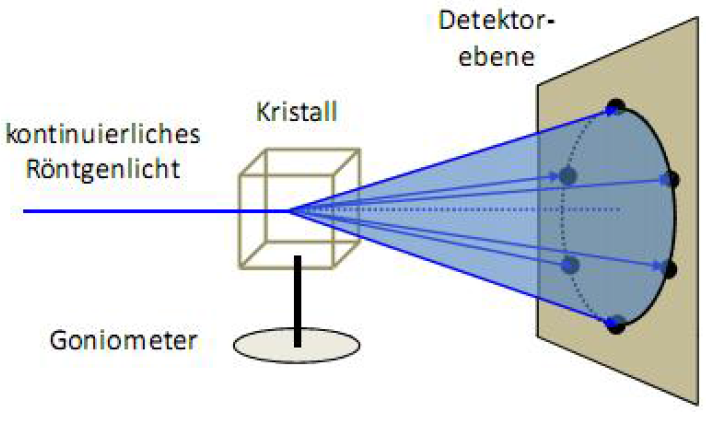
\includegraphics[width = 0.8\textwidth]{laueauf.png}
		\caption{Schematic illustration of Laue method}
		\label{laueauf}
	\end{figure}
	The Laue method is based on a continuous X-Ray beam. According to the circumstances of the sample width, the image plates are positioned in front or behind the sample. The Laue method is schematically illustrated in figure \ref{laueauf}. The figure shows the case of front scattering. The case of backscattering is relatively similar to the case of front scatter. Here it differs in two ways. The first is that the X-Ray beam has to pass the imaging plate through a hole on the plate lane. The second thing is, that one detects the backscattered intensity on the plates. If one would work with a monochromatic beam, one has to guarantee a very good adjustment of the crystal to get diffraction reflexes. To avoid adjustment problems one can use a broad spectrum of x-rays to fulfill the Bragg condition. This method allows one to measure and determine crystal symmetries and orientations.
	
	\subsection{Plane film}
	In this part of the experiment we use monochromatic X-Rays. The X-Rays source beam is conducted through a monochromator to ensure a monochromatic beam. Afterwards the beam is focused to the sample with a collimator. The used set-up requires a sample mounted immediately behind the collimator. The mounting is realized with sticky tape. Notice that the tape induces diffraction reflexes too. In order to eliminate these, a diffraction pattern of the tape itself is taken as reference. To avoid damaging of the imaging plates further we used a beamstopper to decrease the incident beam intensity.
	
	\subsection{Guinier - camera}
	\begin{figure}
		\centering
		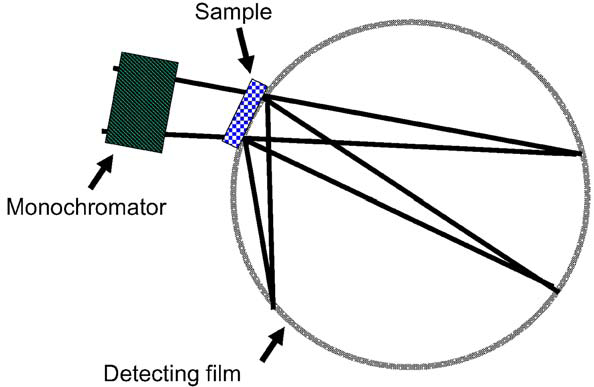
\includegraphics[width=0.8\textwidth]{Guinier.png}
		\caption[Schematic illustration of a Guinier- camera]{Schematic illustration of a Guinier- camera. Notice that the sample rotates around its surface vector.}
		\label{Guinier}
	\end{figure}
	In figure \ref{Guinier} shows a schematic illustration of a Guinier- camera. The sample lies on a rotatable plate. This plate rotates along his surface vector. The rotation speed $\omega$ stays constant. After hitting the sample with the incident X-Ray beam, the image film detects the diffraction pattern. The principle of a Guinier- camera is similar to the Debye-Scherrer method, but initially with two differences. Obviously the first main difference is a solid sample in the Guinier method. The Debye-Scherrer method works with small crystalline powders. The second difference is the result of diffraction pattern. In case of Debye-Scherrer method one gets a diffraction rings imaged on a curved imaging plate. Actually restricted two the spacial dimension of the imaging plate, one gets a small part of the diffraction rings. Further these show a curvature. In case of Guinier the diffraction result is based on sharp non curved lines. Further in this experimental part we used a beamstopper for intensity decreasing. The camera is also evacuated to avoid air scattering. For distinguishing scattering reflexes and main beam there is been taken a measurement without a beamstopper.
